\documentclass[11pt]{article}

\usepackage{tikz}
\usetikzlibrary{patterns}
\usetikzlibrary{snakes}
\usetikzlibrary{trees}
\usetikzlibrary{shapes.callouts}
\usetikzlibrary{shadows}
\usetikzlibrary{matrix}
\usetikzlibrary{shapes.geometric}
\usetikzlibrary{shapes.symbols}
\usetikzlibrary{shapes.arrows}
\usetikzlibrary{shapes.misc}
\usetikzlibrary{calc}
\usepackage{kotex}

\usetikzlibrary{arrows.meta}

\newcommand{\mytikzarea}{%
\draw[step=0.5cm, color=lightgray, thin] (0,0) grid (5.2, 2.7);
\draw[fill=green, opacity=0.5] (15:3) arc (15:45:3) -- (0,0) -- cycle;
\draw[dotted, thin] (2.5, 1.35) circle (1);}

\begin{document}
Hello world? One

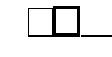
\begin{tikzpicture}
\tikz{\draw (0,0) rectangle (2ex, 1em)}
\tikz[very thick] \draw (0,0) rectangle (2ex, 1em); \\
\tikz \draw (0pt, 3pt) -- (20pt, 3pt);
\end{tikzpicture}

\begin{tikzpicture}
\tikz \draw (0pt, 3pt) -- (20pt, 3pt);
\end{tikzpicture}

\begin{tikzpicture}
\tikz \draw[>-] (0pt, 3pt) -- (20pt, 3pt);
\end{tikzpicture}

\begin{tikzpicture}
\tikz \draw[->] (0pt, 3pt) -- (20pt, 3pt);
\end{tikzpicture}

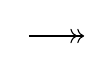
\begin{tikzpicture}
\tikz \draw[->>] (0pt, 3pt) -- (20pt, 3pt);
\end{tikzpicture}

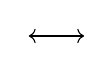
\begin{tikzpicture}
\tikz \draw[<->] (0pt, 3pt) -- (20pt, 3pt);
\end{tikzpicture}

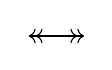
\begin{tikzpicture}
\tikz \draw[<<->>] (0pt, 3pt) -- (20pt, 3pt);
\end{tikzpicture}

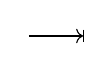
\begin{tikzpicture}
\tikz \draw[->|] (0pt, 3pt) -- (20pt, 3pt);
\end{tikzpicture}

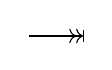
\begin{tikzpicture}
\tikz \draw[->>|] (0pt, 3pt) -- (20pt, 3pt);
\end{tikzpicture}

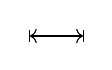
\begin{tikzpicture}
\tikz \draw[|<->|] (0pt, 3pt) -- (20pt, 3pt);
\end{tikzpicture}

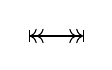
\begin{tikzpicture}
\tikz \draw[|<<->>|] (0pt, 3pt) -- (20pt, 3pt);
\end{tikzpicture}

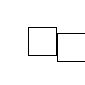
\begin{tikzpicture}
\tikz \draw (0,0) rectangle (1em, 1em);
\tikz[baseline=2pt] \draw (0, 0) rectangle (1em, 1em);
\end{tikzpicture}

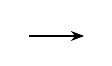
\begin{tikzpicture}
\tikz \draw[-Stealth] (0pt, 3pt) -- (20pt, 3pt);
\end{tikzpicture}

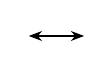
\begin{tikzpicture}
\tikz \draw[Stealth-Stealth] (0pt, 3pt) -- (20pt, 3pt);
\end{tikzpicture}

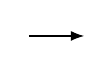
\begin{tikzpicture}
\tikz \draw[-Latex] (0pt, 3pt) -- (20pt, 3pt);
\end{tikzpicture}

\begin{tikzpicture}
\tikz \draw[-{Classical TikZ Rightarrow}] (0pt, 3pt) -- (20pt, 3pt);
\end{tikzpicture}

\tikz{\draw[-{Stealth[length=3mm]}](0,0)--(1.2,0);
\draw[|<->|](0.8,.4) -- node[above=1mm]{3mm}(1.2,.4);}

\tikz{\draw[-{Latex[length=3mm]}](0,0)--(1.5,0);
\draw[|<->|](0.8,.4) -- node[above=1mm]{3mm}(1.2,.4);}

\tikz{\draw[-{Classical TikZ Rightarrow [length=3mm]}](0,0)--(1.2,0);
\draw[|<->|](0.8,0.6) -- node[above=1mm]{3mm}(1.2,.6);}

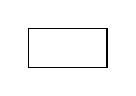
\begin{tikzpicture}
\draw rectangle (1,0.5);
\end{tikzpicture}

\begin{tikzpicture}[x=2, y=1, z=2]
\draw rectangle (2,3);
\end{tikzpicture}

\begin{tikzpicture}[x={(2mm,0)}, y={(0,1mm)}]
\draw rectangle (2,3);
\end{tikzpicture}

\tikz{\draw[line width=5pt] (0,0) -- (1cm, 1.5ex);}
\tikz{\draw[ultra thin] (0,0) -- (1cm,1.5ex);}
\tikz{\draw[very thin] (0,0) -- (1cm, 1.5ex);}
\tikz{\draw[thin] (0,0) -- (1cm,1.5ex);}
\tikz{\draw[semithick] (0,0) -- (1cm, 1.5ex);}

\tikz{\draw[thick] (0,0) -- (1cm, 1.5ex);}
\tikz{\draw[very thick] (0,0) -- (1cm, 1.5ex);}
\tikz{\draw[ultra thick] (0,0) -- (1cm, 1.5ex);}
\tikz{\draw[dash pattern=on 20pt off 3pt on 4pt off 4pt] (0pt, 0pt) -- (50pt, 8pt);}
\tikz{\draw[dash pattern=on 20pt off 8pt, dash phase=0pt](0pt, 0pt) -- (50pt, 8pt);}

\tikz{\draw[dash pattern=on 20pt off 8pt, dash phase=10pt](0pt, 0pt) -- (50pt, 8pt);}
\tikz{\draw[solid](0pt, 0pt) -- (50pt, 8pt);}
\tikz{\draw[dotted](0pt, 0pt) -- (50pt, 8pt);}
\tikz{\draw[densely dotted](0pt, 0pt) -- (50pt, 8pt);}
\tikz{\draw[loosely dotted](0pt, 0pt) -- (50pt, 8pt);}

\tikz{\draw[dashed](0pt, 0pt) -- (50pt, 8pt);}
\tikz{\draw[densely dashed](0pt, 0pt) -- (50pt, 8pt);}
\tikz{\draw[loosely dashed](0pt, 0pt) -- (50pt, 8pt);}
\tikz{\draw[dash dot](0pt, 0pt) -- (50pt, 8pt);}
\tikz{\draw[densely dash dot](0pt, 0pt) -- (50pt, 8pt);}

\tikz{\draw[loosely dash dot](0pt, 0pt)--(50pt, 8pt);}
\tikz{\draw[dash dot dot](0pt, 0pt) -- (50pt, 8pt);}
\tikz{\draw[densely dash dot dot](0pt, 0pt) -- (50pt, 8pt);}
\tikz{\draw[loosely dash dot dot](0pt, 0pt) -- (50pt, 8pt);}

\begin{tikzpicture}[x=1cm, y=1cm]
\draw[thick, ->] (0,0) -- (5,0); % x 축
\draw[very thick, ->] (2.5, -2.5) -- (2.5, 2.5); % y 축
\draw[color=red](2.5, 0) circle (1.5);
\end{tikzpicture}

\begin{tikzpicture}[scale=1.1]
\draw node[rectangle, draw] at (0,0) {노드};
\shadedraw[draw] (2,0) circle [x radius=0.8, y radius=1];
\shade[color=white] (4,0) circle [x radius=0.8, y radius=1];
\fill[pink, draw] (6,0) circle [x radius=0.8, radius=1];
%\pattern[pattern=horizontal lines light blue, draw] (8,0) ellipse [x radius=0.8, y radius=1];
\end{tikzpicture}

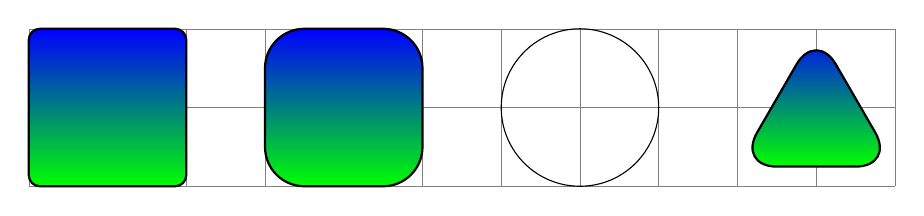
\begin{tikzpicture}
\tikzstyle mystyle=[style={thick, shade, top color=blue, bottom color=green, rounded corners=.5cm}];
\draw[help lines] (0,0) grid (11,2);
\draw[style=mystyle, rounded corners] (0,0) rectangle (2,2);
\draw[style=mystyle] (3,0) rectangle (5,2);
\draw[rounded corners=1cm](6,0) rectangle (8,2);
\draw[style=mystyle] (9, 0.25) -- (11, 0.25) -- (10, 1.98) -- cycle;
\end{tikzpicture}

\begin{tikzpicture}[scale=1.3]
\draw[step=1cm, gray!70, thin] (0,0) grid (4.2, 2.2);
\draw[thick, <->] (0, 2.2) -- (0,0) -- (4.2,0);
\draw[fill, green] (2,1) circle [radius=2pt];

\node[text=red, font=\Large\bfseries] at (2,1){기본};
\node[below=3mm] at (2,1) {아래};
\node[above=2mm] at (2,1) {위쪽};
\node[left=.5cm] at (2,1) {왼쪽};
\node[right=.5cm] at (2,1) {오른쪽};
\end{tikzpicture} \\
%%
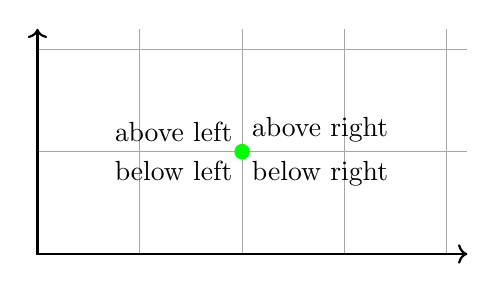
\begin{tikzpicture}[scale=1.3]
\draw[step=1cm, gray!70, thin] (0,0) grid (4.2, 2.2);
\draw[thick, <->] (0,2.2) -- (0,0) -- (4.2,0);
\draw[fill, green] (2,1) circle [radius=2pt];

\node[above left] at (2,1) {above left};
\node[above right] at (2,1) {above right};
\node[below left] at (2,1) {below left};
\node[below right] at (2,1) {below right};
\end{tikzpicture}

\begin{tikzpicture}[xscale=1.3]
\draw[step=3cm, gray!70, thin] (0, -0.2) grid (9, 0.2);
\node[align=left, below] at (1.5, -0.5){이 부분은 \\ 왼쪽으로 \\정렬되지 않을까요?};
\node[align=center, below] at (4.5, -0.5) {이 부분은\\중앙으로 \\정렬되지 않을까요?};
\node[align=right, below] at (7.5, -0.5) {이 부분은\\오른쪽으로 \\정렬되지 않을까요?};
\end{tikzpicture}

\begin{tikzpicture}
\node[fill=pink] at (0, 0) {상자};
\node[draw] at (1.5, 0) {긴 상자};
\node[draw] at (4,0) {좀 더 긴 상자};
\node[fill=pink, circle] at (6,0) {원};
\node[fill=pink, circle] at (7.5cm, 0) {중간 원};
\node[fill=pink, circle] at (9.5cm, 0) {제일 큰 원};
\end{tikzpicture}

\begin{tikzpicture}
\draw node[fill=yellow, draw, circle, text width=1.5cm] at (0,0) {원};
\draw node[fill=yellow, draw, circle, text width=1.5cm] at (2,0) {중간 원};
\draw node[fill=yellow, draw, circle, text width=1.5cm] at (4,0) {큰 원};
\draw node[fill=pink, draw=blue, circle, text width=1.5cm, align=center] at (6,0) {원};
\draw node[fill=pink, draw=blue, circle, text width=1.5cm, align=center] at (8,0) {중간 원};
\draw node[fill=pink, draw=blue, circle, text width=1.5cm, align=center] at (10,0) {큰 원};
\end{tikzpicture}

\begin{tikzpicture}[scale=1.3]
\node[rectangle, draw] at (0,0) {사각형};
\node[rectangle, draw, minimum size=2cm] at (2,0) {사각형};
\node[circle, draw, minimum size=2cm] at (2,0) {};
\node[rectangle, draw, inner sep=2ex] at (4,0) {사각형};
\end{tikzpicture}

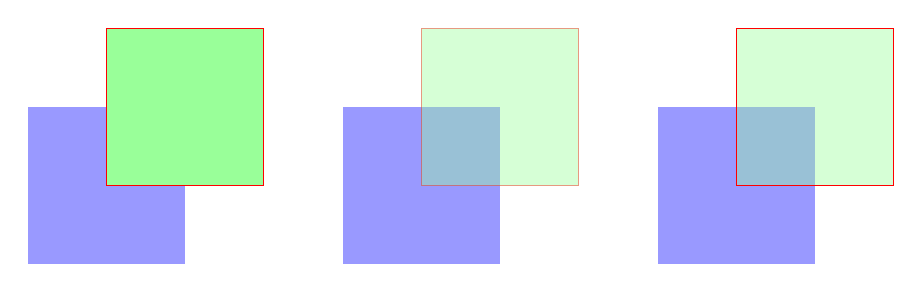
\begin{tikzpicture}
\fill[color=blue!40] (0,0) rectangle (2,2);
\fill[green!40, draw=red] (1,1) rectangle (3,3);
\fill[blue!40] (4,0) rectangle (6,2);
\fill[green!40, draw=red, opacity=0.4] (5,1) rectangle (7,3);
\fill[blue!40] (8,0) rectangle (10,2);
\fill[green!40, draw=red, fill opacity=0.4] (9,1) rectangle (11,3);
\end{tikzpicture}

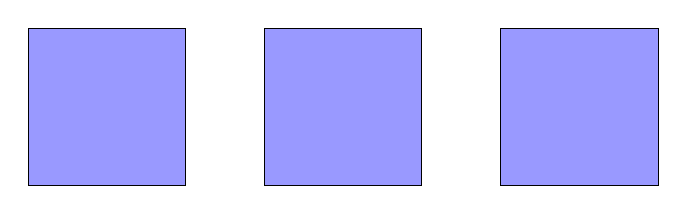
\begin{tikzpicture}
\filldraw[fill=blue!40, draw=black](0,0) rectangle (2,2);
\fill[blue!40](3,0) rectangle (5,2);
\draw[black](3,0) rectangle (5,2);
\fill[color=blue!40, draw=black] (6,0) rectangle (8,2);
\end{tikzpicture}

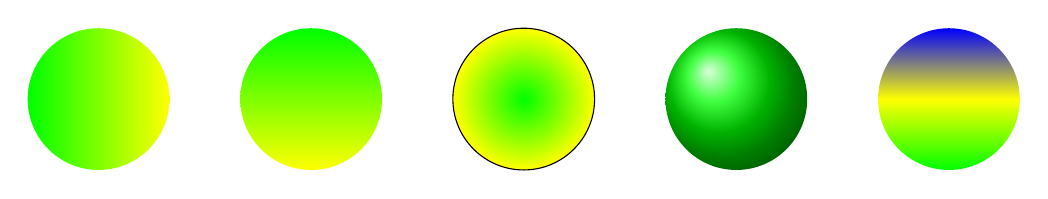
\begin{tikzpicture}[scale=.9]
\shade[left color=green, right color=yellow] (0,0) circle (1);
\shade[top color=green, bottom color=yellow] (3,0) circle (1);
\shade[inner color=green, outer color=yellow, draw=black] (6,0) circle (1);
\shade[ball color=green] (9,0) circle [radius=1];
\shade[top color=blue, bottom color=green, middle color=yellow] (12,0) circle [radius=1];
\end{tikzpicture}

%\begin{tikzpicture}[scale=0.8]
%\shade[shading=color wheel] (0,0) circle (1.5);
%\fill[white] (4,0) circle (1);
%\shade[shading=color wheel black center] (8,0) circle (1.5);
%\end{tikzpicture}

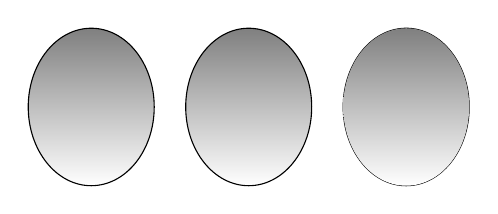
\begin{tikzpicture}
\draw[shade] (2,0) circle [x radius=0.8, y radius=1];
\shadedraw (4,0) circle [x radius=0.8, y radius=1];
\draw (6,0) ellipse [x radius=0.8, y radius=1];
\shade (6,0) circle [x  radius=0.8, y radius=1];
\end{tikzpicture}

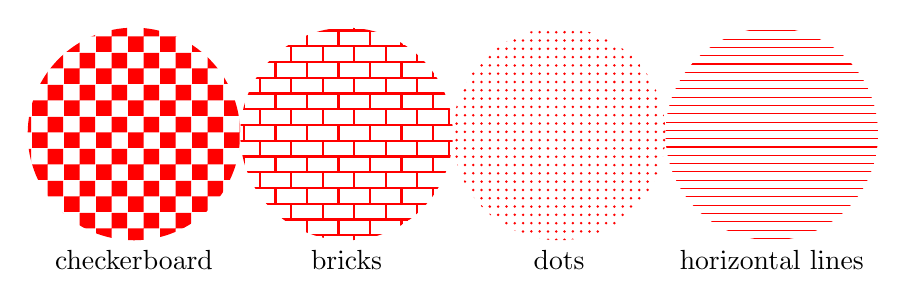
\begin{tikzpicture}[scale=0.9]
\foreach \x/\y in {0/checkerboard, 3/bricks, 6/dots, 9/horizontal lines}{
\pattern[pattern color=red, pattern=\y](\x,0) circle [radius=1.5];
\node[below] at (\x, -1.5) {\y};};
\end{tikzpicture}

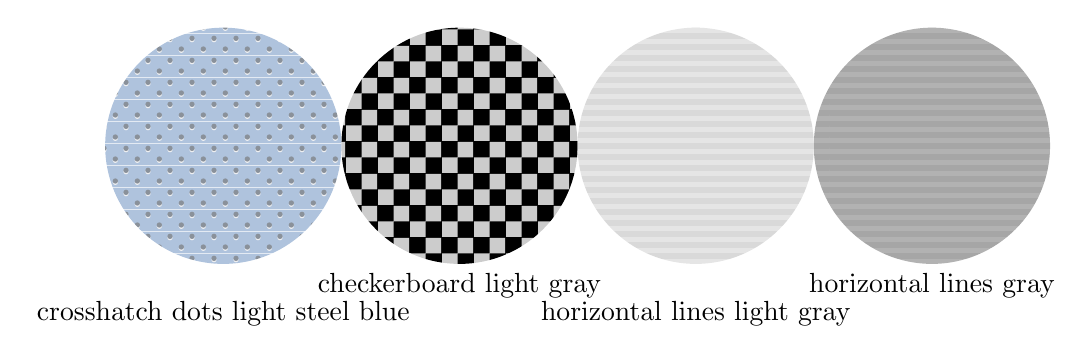
\begin{tikzpicture}
\foreach \x/\y in {3/checkerboard light gray, 9/horizontal lines gray} {\pattern[pattern color=red, pattern=\y] (\x,0) circle [radius=1.5];
\node[below] at (\x, -1.5) {\y};};
\foreach \x/\y in {0/crosshatch dots light steel blue, 6/horizontal lines light gray}{\pattern[pattern=\y] (\x,0) circle [radius=1.5];
\node[below=1em] at (\x, -1.5) {\y};};
\end{tikzpicture}

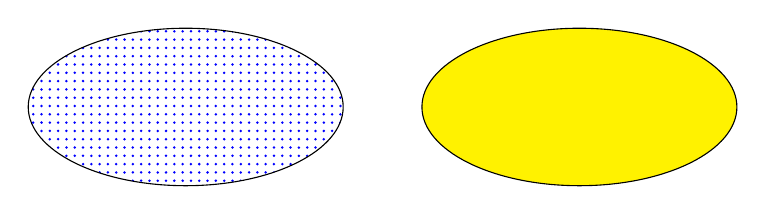
\begin{tikzpicture}
\draw[fill=yellow, pattern color=blue, pattern=dots] (0,0) ellipse (2 and 1);
\draw[pattern color=blue, pattern=dots, fill=yellow] (5,0) ellipse (2 and 1);
\end{tikzpicture}

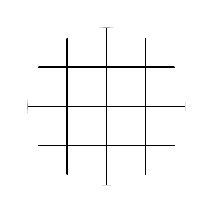
\begin{tikzpicture}
\clip (2,1) circle (1);
\draw[step=0.5cm] (0,0) grid (4,3);
\end{tikzpicture} \hspace{2cm}

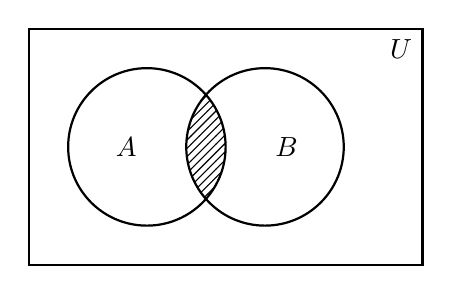
\begin{tikzpicture}[thick]
\draw (0,0) rectangle (5,3) node[below left]{$U$};
\draw (1.5,1.5) circle (1cm) node[left] {$A$};
\draw (3,1.5) circle (1cm) node[right] {$B$};
\begin{scope} % 교집합
\clip (3,1.5) circle (1cm);
\pattern[pattern=north east lines] (1.5,1.5) circle (1cm);
\end{scope} % end scope
\end{tikzpicture} 

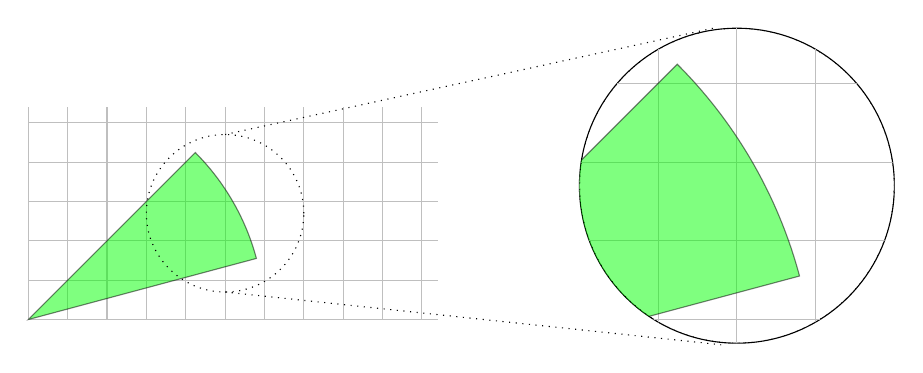
\begin{tikzpicture}
\mytikzarea
\draw[thin, dotted] (2.5, 0.35) -- (8.8, -0.32) (2.5, 2.35) -- (8.7, 3.7);
\begin{scope}[xshift=4cm, yshift=-1cm, scale=2]
\clip[draw] (2.5, 1.35) circle (1);
\mytikzarea
\end{scope}
\end{tikzpicture}

\begin{tikzpicture}
\begin{scope}
\path node at (0,0) (sw) {} node at (3,3) (ne) {}; % 좌표 이름만 설정

\draw (sw) -- (ne);
\shade[ball color=green] (sw) circle (1) (ne) circle (1);
\draw[color=white] (sw) node {남서} (ne) node {북동};
\end{scope}

%% 두 번째 그림
\begin{scope}[scale=1.4, xshift=6cm, yshift=1cm]
\draw[->, very thick] (-2,0) -- (2,0); % x축
\draw[->, very thick] (0,-2) -- (0,2); % y축
\draw[blue, domain=-1.5:1.5] plot (\x, {1-pow(\x,2)});
%\path[name path=x axis] (-2,0) -- (2,0); % x축

%\path[domain=-1.5:0, name path=left curve] plot (\x, {1-pow(\x,2)});
%\draw[thick, oragne, name intersections={of=x axis and left curve, by=x}] (x) -- (0,1);

%\path[domain=0:1.5, name path=right curve] plot (\x, {1-\x*\x});
%\draw[thick, orange, name intersections={of=x axis and right curve, by=y}] (0,1) -- (y);
\end{scope}
\end{tikzpicture}

\begin{tikzpicture}
\draw[->, draw, thick] (-0.5,0) -- (6,0); % x축
\draw[->, draw, thick] (0,-0.5) -- (0,5); % y축
\path[draw] (2.5, 2.1) circle [radius=2cm];

%\path[draw, name path=deg30line] (0,0) -- (30:7); % 30도
%\path[draw, name path=deg60line] (0,0) -- (60:6); % 60도

%\draw[fill=green, name intersections={of=deg30line and mcircle, total=\npoints}] \foreach \i in {1,...,\npoints} {(intersection-\i) coordinate (deg30pts-\i) (deg30pts-\i) circle (3pt)};
%\draw[name intersections={of=deg60line and mcircle, total=\npoints}] \foreach \i in {1,...,\npoints} {(intersection-\i) coordinate (deg60pts-\i)};

%\draw[fill=green] (deg60pts-1) circle (3pt);
%\draw[fill=green] (deg60pts-2) circle (3pt);

%\draw[dotted] (deg60pts-1) -- (deg30pts-1) (deg30pts-2) -- (deg60pts-2);
\end{tikzpicture}

왼쪽

\begin{tikzpicture}[thick]
\draw[blue] (1,0) -- ++(3em, 2ex);
\end{tikzpicture}
오른쪽

왼쪽
\begin{tikzpicture}[thick]
\useasboundingbox
(0,0) rectangle (1,.5);
\draw[blue] (1,0) -- ++(3em, 2ex);
\end{tikzpicture}
오른쪽

왼쪽
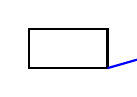
\begin{tikzpicture}[thick]
\draw[use as bounding box] (0,0) rectangle (1,.5);
\draw[blue] (1,0) -- ++(3em, 2ex);
\end{tikzpicture}
오른쪽

왼쪽

\begin{tikzpicture}[thick]
\useasboundingbox (0,0) rectangle (0,0);
\draw[blue] (0,0) -- (3em, 2ex);
\end{tikzpicture}
오른쪽

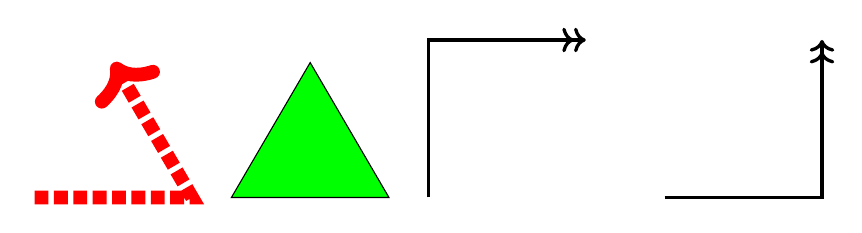
\begin{tikzpicture}
\draw[red, dotted, line width=5pt, ->] (0,0) -- (2,0) -- (1,1.713);
\draw[fill=green] (2.5,0) to (4.5,0) to (3.5, 1.713) to cycle;
\draw[very thick, ->>] (5,0) |- ++(2,2);
\draw[very thick, ->>] (8,0) -| ++(2,2);
\end{tikzpicture}

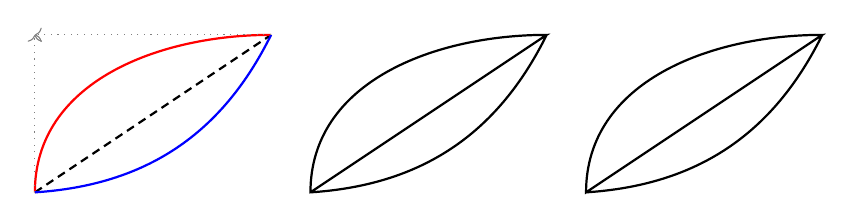
\begin{tikzpicture}
\draw[densely dashed, thick] (0,0) to (3,2);
\draw[red, thick] (0,0) to [out=90, in=180] (3,2);
\draw[blue, thick] (0,0) to [bend right] (3,2);
%% 가이드 가인
\draw[dotted, gray, ->] (0,0) -- (0,2);
\draw[dotted, gray, ->] (3,2) -- (0,2);
%% x축으로 3.5 이동해 다시  그림.
\draw[thick] (3.5,0) to (6.5,2) to [out=180, in=90] (3.5,0) to [bend right] (6.5, 2);
%% x축으로 7 이동해 다시 그림.
\draw[thick] (7,0) to (10,2) to [out=180,in=90] cycle to [bend right] (10,2);
\end{tikzpicture}

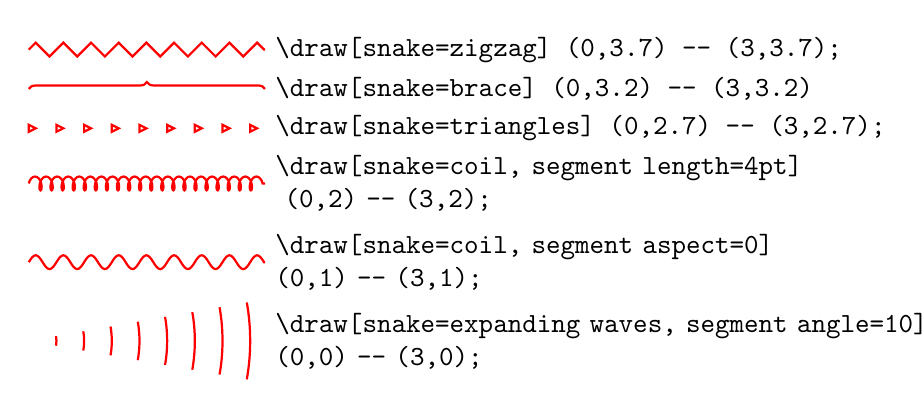
\begin{tikzpicture}[thick]
\draw[red, snake=zigzag] (0,3.7) -- (3,3.7) node[black, right] {\verb|\draw[snake=zigzag] (0,3.7) -- (3,3.7);|};
\draw[red, snake=brace] (0,3.2) -- (3,3.2) node[black, right] {\verb|\draw[snake=brace] (0,3.2) -- (3,3.2)|};
\draw[red, snake=triangles] (0,2.7) -- (3,2.7) node[black, right] {\verb|\draw[snake=triangles] (0,2.7) -- (3,2.7);|};
\draw[red, snake=coil, segment length=4pt] (0,2) -- (3,2) node[black, right, text width=7cm] {\verb|\draw[snake=coil, segment length=4pt]| \\ \verb| (0,2) -- (3,2);|};
\draw[red, snake=coil, segment aspect=0] (0,1) -- (3,1) node[black, right, text width=7cm] {\verb|\draw[snake=coil, segment aspect=0]| \\ \verb|(0,1) -- (3,1);|};
\draw[red, snake=expanding waves, segment angle=10] (0,0) -- (3,0) node[black, right, text width=7cm] {\verb|\draw[snake=expanding waves, segment angle=10]|\\ \verb|(0,0) -- (3,0);|};
\end{tikzpicture}

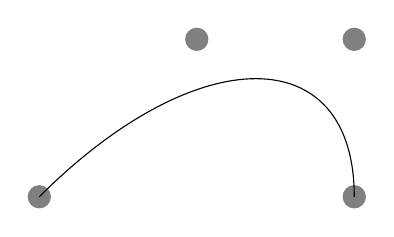
\begin{tikzpicture}[scale=2]
\filldraw[gray] (0,0) circle (2pt)
				(1,1) circle (2pt)
				(2,1) circle (2pt)
				(2,0) circle (2pt);
\draw (0,0) .. controls (1,1) and (2,1) .. (2,0);
\end{tikzpicture}
\, \,
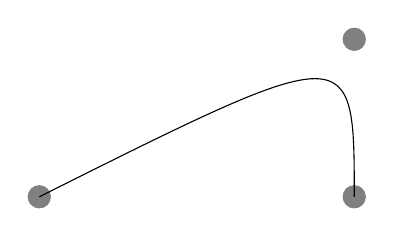
\begin{tikzpicture}[scale=2]
\filldraw [gray] (0,0) circle (2pt)
			     (2,1) circle (2pt)
			     (2,0) circle (2pt);
\draw (0,0) .. controls (2,1) .. (2,0);
\end{tikzpicture}

\begin{tikzpicture}
\draw[dotted, thick] (0,0) rectangle (2,2);
\draw (1,1) circle (1cm);
\draw (1,2) arc (0:180:.8cm); % 원의 왼쪽 호
\draw (1,2) arc[start angle=180, end angle=0, radius=.8cm];
\fill (1,1) circle (2pt); % 중심 표시

\draw[dotted, thick] (3,0) rectangle (7,2);
\draw (5,1) ellipse (2cm and 1cm);
\draw (7,1) arc (180:0:2cm and 1cm); % 타원의 호
\fill (5,1) circle (2pt); % 중심 표시
\end{tikzpicture}

\begin{tikzpicture}
\draw[->] (-0.3,0) -- (2*pi+.3,0); %x축
\draw[->] (0,-1.3) -- (0, 1.3); % y축
%\draw[green, domain=-0.2:2*pi] plot (\x, {sin(\x, r)});
%\draw[red, domain=-0.2:2*pi] plot (\x, {cos(\x, r)});
\end{tikzpicture}

\begin{tikzpicture}[xscale=0.6]
\draw[->, thick] (-pi,0) -- (pi,0); % x축
\draw[->, thick] (0,-1.2) -- (0, 1.2); % y 
%\draw[magenta] plot file {sin.dat};

\tikzset{xshift=6.5cm};
\draw[->, thick] (-pi,0) -- (pi,0); % x축
\draw[->, thick] (0, -1.2) -- (0, 1.2); % y축
%\draw[blue] plot[smooth] file {sin.dat};  

\tikzset{xshift=6.5cm}; 
\draw[->, thick] (-pi, 0) -- (pi,0); % x축
\draw[->, thick] (0,-1.2) -- (0, 1.2); % y축
%\draw[green] plot[only marks, mark] file {sin.dat};
\end{tikzpicture}

\begin{tikzpicture}
\draw (2,0) grid (5.8,2.8);
\draw[step=0.5cm, gray, very thin] (0,0) grid (2.8,2.8);
\draw (6,0) grid [step=0.5, gray, very thin] (8.8, 2.8);
\draw [help lines] (9,0) grid (11.8,2.8);
\end{tikzpicture}

\begin{tikzpicture}
\draw[help lines] (-1,-1) grid (2.4,4.4);
\draw[red] (-1,1) parabola bend (0,0) (2,4); % 왼쪽

\tikzstyle shifted=[xscale=1.5, xshift=4cm, thick];
\shade[style=shifted, top color=green] (0,0) -- (0,4) parabola (2,0) -- cycle; % 적분 영역
\draw[style=shifted, ->] (-1,0) -- (3.0, 0) node[below] {$x$}; % x축
\draw[style=shifted, ->] (0,-0.5) -- (0,4.5) node [left] {$y$}; % y
\draw[style=shifted, blue] (-1, 3) parabola bend (0,4) (2.2, -0.84);
\node[xshift=4cm] at (3.2,1){$\displaystyle\int_0^2f(x)dx$};
\node[xshift=4cm] at (4.5,4) {$f(x) = 4 - x ^2$};
\end{tikzpicture}

\begin{tikzpicture}
\node {부모} child[->] {node {아들}} child {node {딸}};

\begin{scope}[xshift=6cm]
\tikzstyle level 1=[sibling distance=4cm, level distance=2cm]
\tikzstyle level 2=[sibling distance=1.5cm, level distance=1.5cm]

\node {부모}
child {node {아들}
	child {node {손자1}}
	child {node {손자2}}
} % end child
child {node {딸}
    child[dotted] {node[red] {외손자1}}
	child {node {외손자2}}
	child {node {외손자3}}
}; % end child
\end{scope}
\end{tikzpicture}

\begin{tikzpicture}[parent anchor=east, child anchor=west, grow=east, color=red, scale=0.9]
\tikzset{%
level 1/.style={sibling distance=1.7cm, level distance=2cm},
level 2/.style={sibling distance=0.7cm, level distance=2cm}}

\begin{scope}
\node[left] {부모}
child {node {아들}
	child {node {손자1}}
	child {node {손자2}}
	}
	
child {node {딸}
	child {node {외손자1}}
	child {node {외손자2}}
	child {node {외손자3}}
	};
\end{scope}

\begin{scope}[xshift=10cm, yshift=1cm, parent anchor=south, child anchor=north, grow=south]
\tikzstyle{every node}=[ball color=magenta, circle, text=white]
\node {부모}
child[->] {node {자녀 1}}
child {node {자녀 2}};
\end{scope}

\begin{scope}[xshift=14cm]
\tikzstyle{every node}=[ball color=magenta, circle, text=white]
\node[text width=1.5cm, align=center]{부모}
child[->] {node {자녀 1}}
child {node {자녀 2}};
\end{scope}
\end{tikzpicture}

\begin{tikzpicture}
\tikzstyle{level 1}=[sibling distance=2cm, level distance=2.5cm]
\tikzstyle{every node}=[ball color=magenta, circle, text=white, text width=1cm, align=center]
\node {부모}
child[->] {node {자녀 1}}
child {node {자녀 2}};
\end{tikzpicture}

\begin{tikzpicture}[edge from parent fork down, scale=2]
\tikzstyle{every node}=[fill=red!30, rounded corners];
\node {부모}
	child {node {자녀 1}}
	child {node {자녀 2}};
\end{tikzpicture}

\begin{tikzpicture}[edge from parent fork down, scale=2]
\tikzstyle{every node}={fill=red!30, rounded corners}
\tikzstyle{edge from parent}=[red, ->, thick, draw]
\node{부모}
	child {node {아들}}
	child {node {딸}};
\end{tikzpicture}

\begin{tikzpicture}[scale=0.75]
\draw[help lines] (0,0) grid (9,6);
\draw (6,2) ellipse (2 and 1);
\draw[fill] (6,2) circle (2pt);

\draw[thick, blue, rotate=45, ->] (6,2) ellipse (2 and 1);
\fill[blue, rotate=45] (6,2) circle (2pt); 

\draw[thick, blue, rotate=45, ->] (0,0) -- (9,0);
\draw[thick, blue, rotate=45, ->] (0,0) -- (0,5);
\draw[thick, blue, ->] (1.5,0) arc (0:45:1.5);
\draw node[right] at (1.5,0.5) {$\theta$};

\draw[red, rotate around={45:(6,2)}] (6,2) ellipse (2 and 1);

\node[ellipse callout, callout absolute pointer={(8,2)}, draw] at (10,1) {기준 타원};
\node[ellipse callout, callout absolute pointer={(2,6.3)}, draw=blue] at (0,7) {전체 회전};
\node[ellipse callout, callout absolute pointer={(7.5,3.3)}, draw=red] at (10,4) {상대 회전};
\end{tikzpicture}

\begin{tikzpicture} [remember picture]
\node[ellipse callout, draw] at (3,2) (ell) {ellipse};
\node[cloud callout, shading=ball, color=white] at (0,4) (cld) {cloud};
\node[rectangle callout, draw] at (0,1) (rect) {rectangle};
\end{tikzpicture} \hspace{2cm}

\begin{tikzpicture} [remember picture]
\tikzstyle costyle=[{ellipse callout, color=white, fill=#1}]
\draw [help lines] grid (4,4);
\node [costyle=red, callout relative pointer={(0,1)}] at (3,1) {상대좌표};
\node [costyle=blue, callout absolute pointer={(0,1)}] at (1,0) {절대좌표};
\node [costyle=green, overlay, callout absolute pointer={(ell.east)}] at (2,3) {외부좌표};
\end{tikzpicture}

\begin{tikzpicture}
\draw[fill=red, drop shadow] (0,0) rectangle (1,1);
\draw[fill=magenta, drop shadow] ++(3,0.5) ellipse (1cm and .5cm);
\draw[fill=blue, copy shadow] ++(5,0) rectangle +(1,1);
\draw [fill=green, double copy shadow] ++(7,0) rectangle +(1,1);
\draw [fill=black, circular glow={fill=red}] ++(9.5,0.5) circle (.5cm);
\end{tikzpicture}

\begin{tikzpicture}[scale=5]
\node [black!20, xshift=0.2ex, yshift=-0.2ex] (0,0) {\bfseries 아주 중요한 일입니다.};
\node [black!40, xshift=0.15ex, yshift=-0.15ex] (0,0) {\bfseries 아주 중요한 일입니다.};
\node [red] (0,0) {\bfseries 아주 중요한 일입니다.};
\end{tikzpicture}

\begin{tikzpicture}
\matrix (mymtx) [matrix of nodes] {
1 & 2 & 3 \\
4 & 5 & 6 \\
7 & 8 & 9 \\
};
\draw[thick, red, ->] (mymtx-1-1) |- (mymtx-2-3);
\end{tikzpicture} \hfill

\begin{tikzpicture}
\matrix [matrix of nodes] {
1 & [5mm] 2 & [1cm] | [blue]| 3 \\
4 &            5 &            | [red]|  6 \\
7 &            8 &                         9 \\};
\end{tikzpicture} \hfill

\begin{tikzpicture} \hfill
\matrix [matrix of nodes] {
1 & 2 & 3 \\
4 & 5 & \node[red, circle, draw] {6}; \\
7 & 8 & \node(0,0) {9}; \draw(0,0) circle [radius=10pt];
\\};
\end{tikzpicture}

\begin{tikzpicture}
\matrix [matrix of math nodes] (three) {
a_{11} & a_{12} & a_{13} = \displaystyle\int f(x) dx \\
a_{21} & a_{22} & |[red]| a_{23} \\
a_{31} & a_{32} & a_{33} \\
};
\draw (three-1-1) node[above=1mm] {\tiny (1,1)번째 원소};
\end{tikzpicture}

\begin{tikzpicture}
\matrix [matrix of math nodes, 
nodes={circle, fill=yellow, draw}] {
a_{11} &  & a_{13} \\
a_{21} & & a_{23} \\
a_{31}  & a_{32} & \\ };
\end{tikzpicture} \hspace{2cm}

\begin{tikzpicture}
\matrix [matrix of math nodes, nodes={circle, fill=yellow, draw},
nodes in empty cells] {
a_{11} & & a_{13} \\
a_{21} & & a_{23} \\
a_{31} & a_{32} & \phantom{a_{33}} \\};
\end{tikzpicture}

\begin{tikzpicture}
\matrix [matrix of nodes, nodes={text width=16mm, draw}] {
1번 행 & {위쪽 줄 \\ 아래쪽 줄} \\
두 번째 & 빈칸 \\};
\end{tikzpicture}

\begin{tikzpicture}
\draw[help lines] (0,0) grid (6,2);
\foreach \x in {0,1,...,6} {
\foreach \y/\tmpcolor in {0/red, 1/green, 2/blue} 
{\fill[\tmpcolor] (\x,\y) circle (2pt);
};
};
\end{tikzpicture}

\begin{tikzpicture}
\draw[help lines, black!20] (-2,0) grid (7,6);
\foreach \x in {-2,-1,...,7} {% x축 눈금
\node[below] at (\x,0) {\small \x}; };
\foreach \y in {0,1,...,6} {% y축 눈금
\node[left] at (-2,\y) {\small \y}; };
\draw[dotted, ->, thick] (0,0) -- (6.2,6.2);
\draw[dotted, ->, thick] (0,0) -- (-2.3, 2.3);
%% 원래 좌표의 경로
\draw[red, ->] (0,1) -- (1,1);
\draw[red] (3,1) circle (1cm);
\fill[red] (3,1) circle (2pt);
\shade[ball color=red] (4.5,2.5) rectangle (5.5,3.5);
%% 기준 벡터 변경
\begin{scope}[x={(1cm, 1cm)}, y={(-2cm, 2cm)}, very thick, blue]
\draw[->] (0,1) -- (1,1);
\draw (3,1) circle (1cm);
\fill (3,1) circle (2pt);
\end{scope}
%% 기준 벡터 변경
\shade[x={(0cm, 1cm)}, y={(1cm, 0cm)}, ball color=green] (4.5,2.5) rectangle (5.5,3.5);
\end{tikzpicture}

\begin{tikzpicture}
\draw (0,0) -- (1,0) -- ([turn]72:1) -- ([turn]72:1) -- ([turn]72:1) -- cycle;
\end{tikzpicture}

\begin{tikzpicture}
\draw[thick] (5,0) rectangle (6,1);
\draw[red, dashed, thick] (3,0) rectangle ++(1,1);
\draw[blue, dotted, thick] (1,0) rectangle +(1,1);
\draw (0,-0.1) -- (+7,-0.1);
\foreach \x in {1,2,3,4,5,6,7} {\draw[thin] (\x, -0.3) node {\x};};
\end{tikzpicture}

\begin{tikzpicture}
\draw   (0,0) node (x) {남서}
			(3,2) node (y) {북동동};
\draw (x) -- (y);

\coordinate (x2) at (4,0);
\coordinate (y2) at (7,2);
\fill [top color=magenta] (x2) rectangle (y2);
\draw[blue, <->] (x2) -- (y2);
\end{tikzpicture}

\begin{tikzpicture}
\node (rect1) at (4,2) [draw=red, ball color=cyan, thick, minimum width=3cm, minimum height=2cm] {};
%% 동서남북
\tikzstyle every node=[draw]; %% 사각형 그리기

\node[right] at (rect1.east) {\texttt{.east}};
\node[below] at (rect1.south) {\texttt{.south}};
\node[left] at (rect1.west) {\texttt{.west}};
\node[above] at (rect1.north) {\texttt{.north}};
%% 모서리 방향
\node[above right] at (rect1.north east) {\texttt{.north east}};
\node[below right] at (rect1.south east) {\texttt{.south east}};
\node[above left] at (rect1.north west) {\texttt{.north west}};
\node[below left] at (rect1.south west) {\texttt{.south west}};
\end{tikzpicture}

\begin{tikzpicture}
\begin{scope}
\coordinate (p1) at (1,1);
\draw [help lines] (0,0) grid (3,2);
\draw [red] ($2*(1,1)$) node {(a)};
\draw [green] (${1+1}*(1,.5)$) node {(b)};
\draw [blue] ($2*(p1)-(1,1.5)$) node {(c)};
\draw [black] (${3*(4-3)}*(1,0.5)$) node {(d)};
\end{scope}
\begin{scope}[xshift=4cm]
\draw [help lines] (0,0) grid (3,2);
\draw[->] (0,0) -- ($1.5*(3,2)$);
\foreach \i in {0,0.5,...,1.5} \node[above] at ($(0,0)!\i!(3,2)$) {\i};
\draw[red] (0,0) -- ($(0,0)!0.5!30:(3,2)$);
\draw[->] ($0.3*(3,2)$) arc (30:60:1);
\end{scope}
\end{tikzpicture}

\begin{tikzpicture}
\draw [help lines] (0,0) grid (4,3);
\coordinate (a) at (0.5,0.5);
\coordinate (b) at (3.5,0.5);
\coordinate (c) at (2.5, 2.5);
\draw (a) -- (b) -- (c) -- cycle;
\draw[red, ->] (c) -- ($(a)!(c)!(b)$);
\draw[blue, ->] (c) -- ($(a)!(c)!90:(b)$);
\node[left] at (a) {\scriptsize A};
\node[right] at (b) {\scriptsize B};
\node[above] at (c) {\scriptsize C};
\draw[green, ->] (b) -- ($(a)!(b)!(c)$);
\draw[blue, ->] (a) -- ($(b)!(a)!(c)$);
\end{tikzpicture}

\begin{tikzpicture}
\node[anchor=south west, inner sep=0] at (0,0) {
\includegraphics[width=0.9\textwidth] {../images/mari.png}};
%
\includegraphics[width=0.9\textwidth] {../images/mari.png}
\node[yellow, right] at (0.5, 6.5) {\bfseries\copyright Songyong Sim};
\draw[help lines] (0,0) grid (12,7);
\draw[blue, very thick, rounded corners] (6.5,2) rectangle (8,2.8);
\end{tikzpicture}

\begin{tikzpicture}
\node[anchor=south west, inner sep=0] (image) at (0,0) {
\includegraphics[width=0.6\textwidth]{../images/mari.png}};
\begin{scope}[x={(image.south east)}, y={(image.north west)}]
\node[yellow, right] at (0.04,0.9) {\scriptsize\copyright Songyong Sim};
\draw[blue, very thick, rounded corners] (0.52,0.28) rectangle (0.62,0.38);
\end{scope}
\end{tikzpicture}

%\begin{tikzpicture}
%\tikzstyle{myImagePath}=[path picture]={\node at (path picture bounding box.center) {\includegraphics[width=6cm]{#1}};}];
%\draw [thick, blue, path picture={\node at (path picture bounding box.center) {
\includegraphics[width=6cm]{../images/mari.png}}}] (0,1) circle (1.5);
%\draw [thick, fill=black!70, patch picture={\node[yellow] at (path picture bounding box.center) {\Large\bf 문자열의 중앙 부분만 가져올까요?};}] (9,1) circle (1.5);
%\end{tikzpicture}

\begin{tikzpicture}
\tikzstyle{my image cut}=[thick, blue, path picture={\node[left=#1] at (path picture bounding box.center){
\includegraphics[width=\textwidth]{../images/mari.png}};}];
\fill[brown] (-0.5,-2.5) rectangle (11.5, 2.5); % 벽돌 색
\draw[pattern=bricks, pattern color=white] (-0.5, -2.5) rectangle (11.5,2.5);
\draw[my image cut=-11cm] (0,-2) rectangle (2,2);
\draw[my image cut=-8cm] (3,-2) rectangle (5,2);
\draw[my image cut=-5cm] (6,-2) rectangle (8,2);
\draw[my image cut=-2cm] (9,-2) rectangle (11,2);
\end{tikzpicture}

\end{document}